\documentclass[11pt]{article}
\usepackage[T1]{fontenc}
\usepackage[french]{babel}
\usepackage{csquotes}
\usepackage[margin=2.5cm]{geometry}
\usepackage{amsmath}
\usepackage{graphicx}
\usepackage{booktabs}
\usepackage[locale=FR]{siunitx}
\usepackage[style=numeric]{biblatex}
\addbibresource{references.bib}
\usepackage[colorlinks=true, allcolors=blue]{hyperref}

\begin{document}

\pagenumbering{alph}
\begin{titlepage}
  \centering
  {\large Établissement \par}
  {\large Département \par}
  \vspace{4cm}
  {\scshape Rapport de laboratoire \par}
  \vspace{1cm}
  {\huge\bfseries {{TITLE}} \par}
  \vspace{2cm}
  {\Large {{AUTHOR}} \par}
  \vspace{1cm}
  Présenté à Nom du professeur \par
  Cours SIGLE1234 \par
  \vfill
  {\large \today \par}
\end{titlepage}
\pagenumbering{arabic}

\tableofcontents
\newpage

\section{Objectifs}

Cette section expose en quelques lignes le but de l'expérience ou du projet
et la question à laquelle il répond.

\section{Matériel et méthode}

\subsection{Matériel}

\begin{itemize}
  \item un oscilloscope numérique;
  \item un générateur de fonctions;
  \item un circuit RC de résistance \qty{10}{\kilo\ohm} et de capacité
        \qty{100}{\nano\farad}.
\end{itemize}

\subsection{Méthode}

On applique une tension en échelon au circuit et on mesure la tension aux
bornes du condensateur. La constante de temps du circuit vaut
\begin{equation}
  \tau = RC = \qty{1}{\milli\second}.
  \label{eq:tau}
\end{equation}

\section{Résultats}

Le tableau~\ref{tab:mesures} rassemble les mesures et la
figure~\ref{fig:resultats} les montre en graphique.

\begin{table}[htbp]
  \centering
  \caption{Tension aux bornes du condensateur.}
  \label{tab:mesures}
  \begin{tabular}{S[table-format=1.1] S[table-format=1.2]}
    \toprule
    {Temps (\unit{\milli\second})} & {Tension (\unit{\volt})} \\
    \midrule
    0,0 & 0,00 \\
    0,5 & 1,97 \\
    1,0 & 3,16 \\
    2,0 & 4,32 \\
    5,0 & 4,97 \\
    \bottomrule
  \end{tabular}
\end{table}

\begin{figure}[htbp]
  \centering
  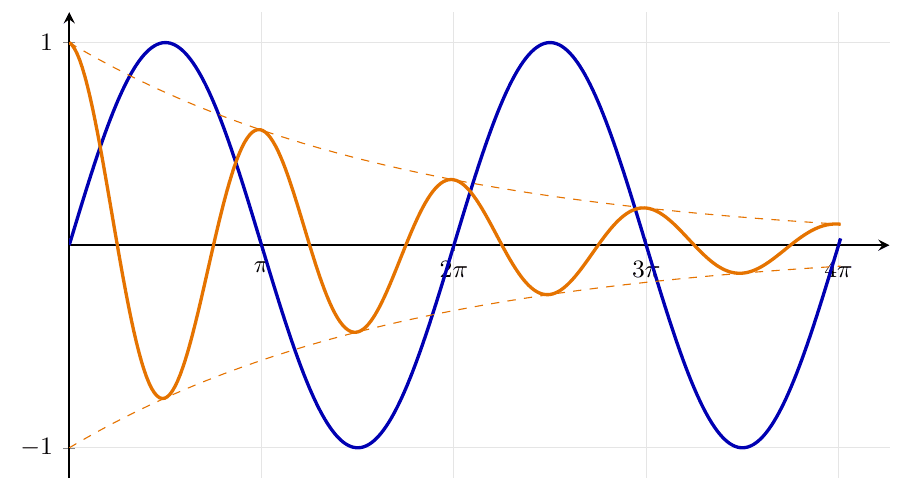
\includegraphics[width=0.75\linewidth]{images/courbes.png}
  \caption{Une image du projet: remplacez-la par vos résultats.}
  \label{fig:resultats}
\end{figure}

\section{Discussion}

On compare les résultats à la théorie de l'équation~\eqref{eq:tau} et on
explique les écarts observés \parencite{taylor1997}.

\section{Conclusion}

La conclusion répond à la question posée dans les objectifs.

\printbibliography[heading=bibintoc]

\appendix
\section{Données brutes}

Les annexes contiennent ce qui alourdirait le rapport: données brutes,
calculs détaillés, code.

\end{document}
